\documentclass{article}
\usepackage{aaai}
\usepackage{graphicx}
\usepackage[ruled, vlined, linesnumbered]{algorithm2e}
\usepackage[toc, page]{appendix}

% Big margins for now so people can take notes/scribbles.
%\usepackage{fullpage}

\title{Parallel Best NBlock First}
\author{Ethan Burns \and Seth Lemons \and Wheeler Ruml \\
  Department of Computer Science \\
  University of New Hampshire \\
  Durham, NH 03824 USA \\
  \{eaburns,seth.lemons, ruml\}@unh.edu}
\date{\today}

\begin{document}
\maketitle

\begin{abstract}
  A lot of work in heuristic search focuses on solving larger and larger
  problems.  Various techniques have been developed for making heuristic
  search more memory efficient.  Other techniques have been developed
  that allow heuristic search to make use of external storage devices
  (such as hard disks) to increase their memory capacity.  In this paper
  we build on some of the techniques used for external memory search to
  create a parallel best-first style search to be used to more quickly
  solve smaller search domains.
\end{abstract}

\section{Introduction}

As microprocessor manufacturers build processors with more and more
cores, software developers are being pressured to create algorithms to
make better use of the newly available parallelism.  In the field of
artificial intelligence it is always necessary to solve problems more
quickly.  A trend in current research on heuristic search, however,
seems to be focusing on finding solutions in larger and larger search
domains instead of solving smaller domains faster.  For this work our
goal was to attempt to use parallelism to solve some problems that are
traditionally considered small more quickly.

There has been a lot previous work in parallel heuristic search.
Various algorithms have been created that exploit features of some
well known search algorithms to concurrently expand portions of a
search graph.  One of the issues that is encountered with parallel
heuristic search, however, is that there is a trade off between
synchronization and performing extra search effort.  This tradeoff can
be directly related to detection of duplicate nodes in the graph.

In a typical, serial best-first search algorithm, an \emph{open-list}
and \emph{closed-list} of nodes are maintained.  The open-list
contains nodes on the search frontier that have yet to be searched
(expanded), and the closed-list maintains nodes which have already
been expanded.  The closed-list is used to detect cycles in the search
graph so that a node is not searched multiple times.  The process of
detection nodes that have already been searched is called
\emph{duplicate detection}.  In a serial best-first search, a node is
added to the closed-list the first time that the search encounters it.
If a node is encountered again during the search process, it is
ignored since it has already been expanded.  This process breaks
cycles and eliminates extra, wasted, search effort.

In a parallel graph search, where many processors are searching nodes
concurrently, keeping track of which nodes have already been searched
can be complicated.  Since multiple processors are searching at the
same time a shared data structure is often necessary to communicate
between the processors which nodes have already been searched.  The
problem with this approach is that the synchronization overhead
required to access a shared data structure can be expensive,
especially as the number of processors increases creating more
contention.  An alternative approach would be to ignore duplicate
tracking altogether, or less extremely, to have each processor only
track duplicate nodes locally; not communicating the information with
other processors at all.  While this approach eliminates
synchronization overhead it leads to extra search effort due to the
searching of nodes that may have already been encountered by other
processors.

External memory graph search is another graph search technique that
exhibits similar problems to those of parallel search.  External
memory graph search uses secondary storage devices, such as a hard
disks, to store large portions of search space which are not currently
being used.  Since secondary storage devices can have a much larger
capacity-per-unit-cost than primary memory, this technique allows
larger search domains to be solved using commonly available hardware.
Both external memory and parallel graph search share a common problem:
duplicate detection must be performed while only having access to a
(possibly small) subset of the entire closed-list.  In the case of
external memory search some of the closed nodes will be residing on a
slow, secondary storage device.  In the case of parallel search some
of the nodes will be in use by other processors.  The question that
must be answered is how to decompose a search graph to allow for
efficient and accurate duplicate detection using only subsets of all
of the graph's nodes.

\section{Previous Work}

\subsection{Parallel Retracting A*}

There has been a handful of algorithms created that attempt to provide
duplicate node detection while reducing the amount of synchronization
between processors.  One such algorithm is Parallel Retracting A*
(PRA*) \cite{evett:pra}.  PRA* attempts to reduce synchronization
overhead by distributing the duplicate detection between processors.
A hashing scheme is used to divide the search nodes up among all of
the available processors.  Each time a processor expands a node,
passes the node to its respective processor based on the hash value of
the node.  Each processor is then in charge of expanding and detecting
duplicates for all of the nodes that hash to it.  This method allows
duplicate detection to happen without communicating between all of the
processors which nodes have already been searched.  The PRA* algorithm
also use a node-retraction scheme to reduce the amount of memory that
a search uses.  For this work, we are only concerned with problems
that fit into memory, and our interest in PRA* is for its unique
method of splitting the search space amongst processors.

One of the problems that PRA* encounters is that, while no
synchronization is required for duplicate detection, there is a
substantial amount of overhead incurred by the message passing that is
used to move nodes to their respective processors.  In a shared memory
system, each processor must have a synchronized queue which all of the
other processors have the ability to add search nodes to.  While this
is less of a bottle-neck than having a single global shared data
structure, we have found that it is still very expensive.

\subsection{Structured Duplicate Detection}

Structured Duplicate Detection or SDD \cite{zhou:sdd} is a method for
performing external memory search.  SDD uses a projection function, a
many-to-one mapping from states in a search space to states in an
abstract space, to decompose a search graph.  The projection function
creates an abstract space of nodes that are projections, or images, of
the nodes in the original state space.  Since the projection function
is a many-to-one mapping, the abstract space is significantly smaller
than the original search space.  For a projection function $p$, $y$ is
said to be the \emph{image} of a node $x$ if $p(x) = y$.  Additionally
$y'$ is a successor of $y$, in the abstract graph, if there are two
states $x$ and $x'$ such that $x'$ is a successor of $x$, $y$ is the
image of $x$ and $y'$ is the image of $x'$.  In other words:

\begin{eqnarray*}
  &&x' \in successors(x) \wedge p(x) = y \wedge p(x') = y' \\
  &\Rightarrow& y' \in successors(y)
\end{eqnarray*}

In the description of the SDD algorithm, Zhou and Hansen use the term
\emph{nblock} to refer to all nodes in the original state space that
have the same image in the abstract space.  Throughout the remainder
of this paper, the terms ``abstract state'', and ``nblock'' will be
used interchangeably, as each nblock corresponds to a single abstract
state.

Zhou and Hansen show that, while performing duplicate detection, only
nodes which reside within the same nblock must be checked for
duplicates.  This is because, for a node $x$ which is a duplicate of a
node $z$, both $x$ and $z$ will project to the same abstract state
(and therefore reside in the same nblock) Intuitively, this makes
sense, because both $x$ and $z$ are the same node.  This leads to the
idea of a \emph{duplicate detection scope}.  By the definition of the
successor set of an abstract node: any child node $x'$ of a node $x$,
in the original state space, will have an image $p(x') \in
successors(p(x))$, and therefore when performing duplicate detection
for $x'$ the only nodes that must be checked are in the nblock $p(x')
\in successors(p(x))$.  For this reason, $successors(p(x))$ is called
the duplicate detection scope of the nblock $p(x)$ -- no other nodes
in the original state space will ever need to be consulted for
duplicate detection when expanding nodes in the nblock $p(x)$.

This idea can be shown using the sliding tile puzzle as an example.
One possible projection function for the sliding tiles puzzle would be
to only look at the position of the empty tile.  For example: all
states with the empty tile in the upper left-hand corner (position 0)
would map to the nblock shown on the left in Figure
\ref{fig:tile-abstraction}, where the grayed square represents the
position of the empty tile.  Using this abstraction, there are sixteen
possible abstract states, one for each possible position of the empty
tile.  It is easy to see that all of the children of a state in the
nblock shown on the left in Figure \ref{fig:tile-abstraction} will
have the empty tile in either position 1 or 4 (either by sliding the
tile in position 1 to the left, or by sliding the tile in position 4
up).  The image on the right, in Figure \ref{fig:tile-abstraction},
shows the duplicate detection scope for the nblock shown on the left
in this figure.  Any of the children of a state in the nblock shown on
the left in Figure \ref{fig:tile-abstraction} will fall into one of
the two nblocks shown on the right.

\begin{figure*}[t]
  \begin{center}
    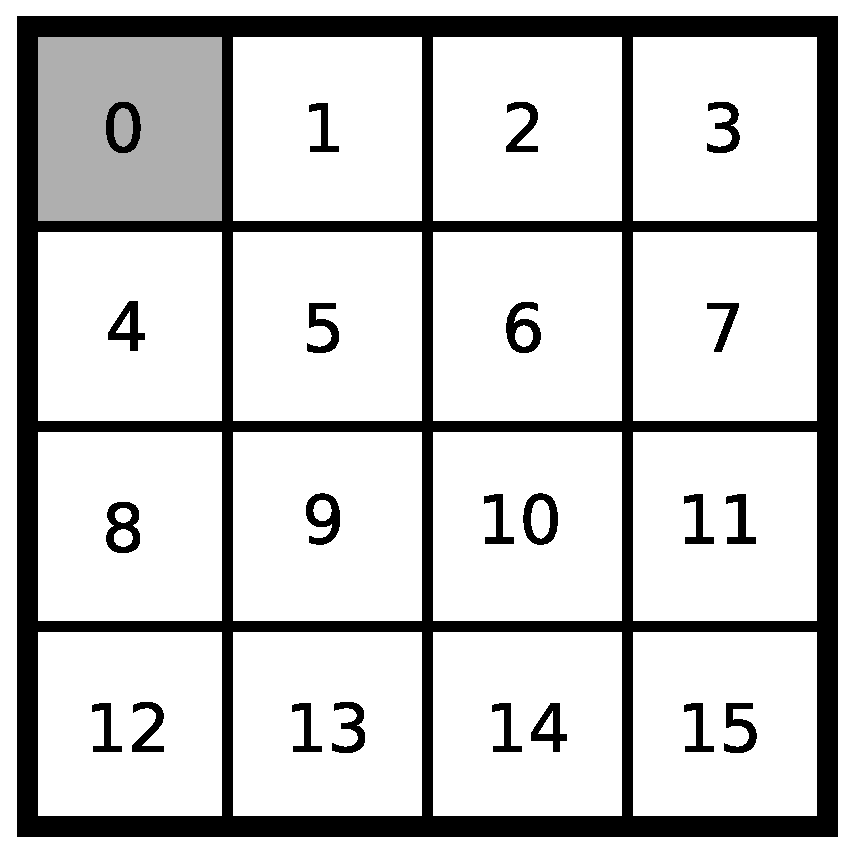
\includegraphics[width=1.5in]{images/tile-abstraction.eps}
    \hspace{4cm}
    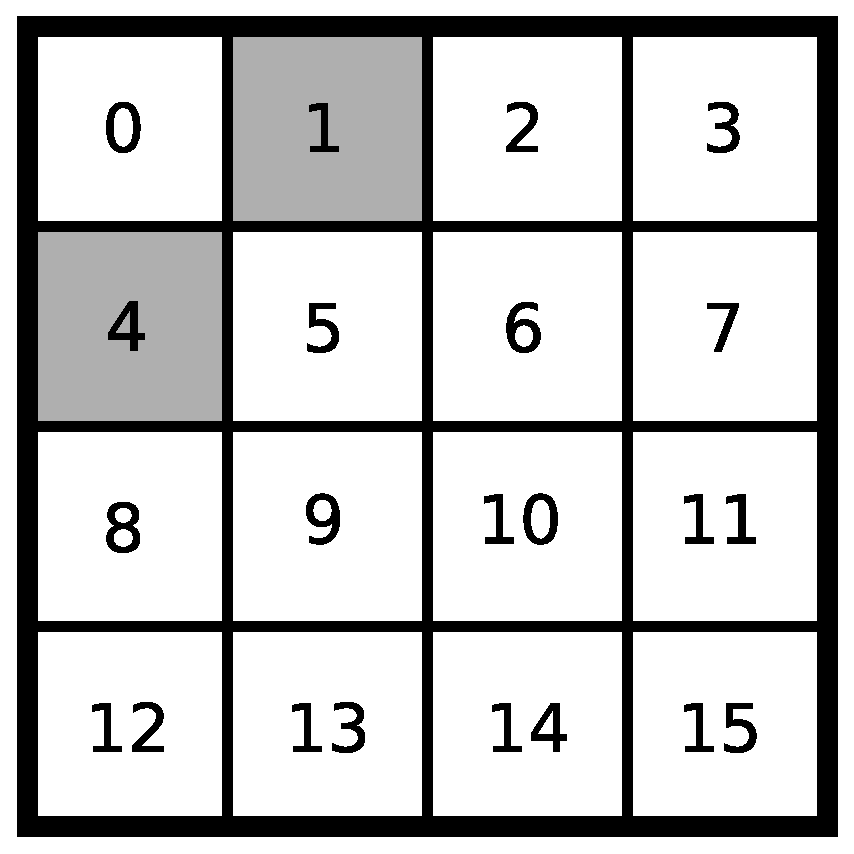
\includegraphics[width=1.5in]{images/duplicate-detection-scope.eps}
    \caption{The abstract image of all states with a empty tile in
      position 0 (left).  The duplicate detection scope of the
      abstract state with the empty tile in position 0 (left).}
    \label{fig:tile-abstraction}
  \end{center}
\end{figure*}

The main focus of the SDD approach is using state space decomposition
so that generated nodes can be explicitly moved to a secondary storage
device (such as a disk drive) when they are not in the duplicate
detection scope of the nblock being expanded and therefore are not
needed.  The SDD approach uses breadth-first heuristic search, where
only the nodes of the current search depth in a single nblock are
searched at a time.  Nodes of this nblock are expanded from the
current depth-layer and their children are placed into the next-depth
layer of their corresponding nblocks.  When the current nblock has no
more nodes at the current depth-layer, it is swapped for another
nblock which does have open nodes at this depth.  If no more nblocks
have nodes at the search depth, the search progresses to the next
layer (which contains the children nodes of the previous layer).  This
procedure repeats until a goal is found, or until no nodes
remain. Since duplicates can only fall into the duplicate detection
scope of the nblock being searched, the remainder of the nodes can be
pushed off to disk, instead of being stored in main-memory.  Nblocks
can then be intelligently swapped into and out of main-memory as the
search progresses.

\subsection{Parallel Structured Duplicate Detection (PSDD)}

While the motivation of SDD is to have explicit control over which
portions of a search space reside in main-memory.  Zhou and Hansen
also show that this approach also lends itself to parallelization
\cite{zhou:psd}.  The parallel SDD (or PSDD) algorithm uses the graph
of nblocks to find \emph{disjoint duplicate detection scopes}, or
duplicate detection scopes that do not overlap.  Nblocks with disjoint
duplicate detection scopes can be searched in parallel without any
locking or contention.  In order to find nblocks with disjoint
duplicate detection scopes the concept of a \emph{free} nblock is
introduced.  An nblock $b$ is considered to be free if no processor is
using an nblock in $successors(b)$ -- in other words, if all other
processors are searching nblocks with duplicate detection scopes which
are disjoint from that of $b$.  Free nblocks are found by tracking a
$\sigma(b)$ value for each nblock $b$, where $\sigma(b)$ is the number
of nblocks in $successors(b)$ that are in use by another processor.
Any nblock $b$ with $\sigma(b) = 0$ is free, and therefore a processor
can acquire $b$ and its duplicate detection scope for a period of lock
free expansion.  Besides tracking disjoint duplicate detection scopes,
the search procedure of PSDD is the same as that of SDD; the search
progresses by searching one depth-layer at a time until a goal is
found or the search space is exhausted.  PSDD is an attractive
algorithm because it reduces the amount of contention between
processors by allowing for lock-free periods of expansion.

\subsubsection{Best-First Parallel Structured Duplicate Detection}



\subsection{Localizing A*}

An alternative approach for improving the efficiency of large searches
is to slightly loosen the node ordering restriction of A* as is done
by Edelkamp and Schrodl \cite{edelkamp:loc}.  Edelkamp and Schrodl
create an algorithm that uses a looser node ordering than A* in order
to achieve a better memory locality. We refer to this algorithm as lA*
(for localized A*).  While lA* expands more nodes than A* does, the
intuition is that lA* can achieve better performance than A* for large
searches because it can reduce the number of virtual-memory operations
that swap to disk.

lA* uses a data structure called a \emph{Heap-of-heaps} to order its
node expansions.  A heap-of-heaps, $H$, is composed of elements $H_0$,
$H_1$, ..., $H_n$, where each element $H_i$ is a heap of search nodes
that reside in the same page of memory.  The heap-of-heaps, $H$, is
loosely sorted based on the f-values of the best nodes of each heap
$H_i$ (denoted as $best(H_i)$).  The lA* procedure searches the best
heap $H_0$, of the heap-of-heaps, until $best(H_1) + \Delta >
best(H_0)$, where $H_1$ is the new best heap on $H$ after the removal
of heap $H_0$.  The $\Delta$ value allows the search to expand a set
of nodes in $H_0$ which may not have a the best f-values, but that
have better memory locality with respect to the previously expanded
nodes.

Since lA* prefers nodes with better memory locality, it reduces the
number of page-faults, and virtual memory swap operations that the
operating system must perform.  The tradeoff is that the first
solution found by lA* may be sub-optimal since it is not searching in
strict f-value order.  To fix this problem, lA* doesn't return its
first solution, instead it behaves like an any-time search algorithm
by continuing the search and pruning on the f-value of incumbent
solutions.  Since the f-value of an incumbent solution is an
upper-bound on the optimal solution, the search can stop when there
are no frontier nodes that have f-values less than the current
incumbent -- this means that the current incumbent solution \emph{is}
the optimal solution.

\section{Parallel Best NBlock First (PBNF)}

One of the nice features of the PSDD algorithm is that it allows
processors to perform periods of lock-free expansions with duplicate
detection.  While this algorithm can perform well, it suffers from
per-layer synchronization.  Each time a layer is complete, all of the
processors must synchronize so that they can all start the next layer
at the same time.  The reason for this in the PSDD algorithm is
because, if processors were to be searching different layers, there
would be a chance that the first solution encountered is not optimal.
A processor searching a further layer may find a solution before a
better solution on a previous layer is found.

In order to get the benefits of lock-free expansion and duplicate
detection that are provided by PSDD without the need for
layer-synchronization, we have created an algorithm that is a
combination of PSDD and lA* called Parallel Best NBlock First (PBNF).
The PBNF algorithm maintains a heap-of-nblocks (this is analogous to
the heap-of-heaps in lA*) and each nblock has a heap of nodes sorted
on f-value.  Processors use the heap-of-nblocks to attempt to acquire
a free nblock with the lowest f-valued search node.  Instead of
releasing an nblock when it no longer contains any more search nodes,
processors \emph{switch} their nblock for a better one as they become
available.

\begin{algorithm}
  \caption{PBNF Search}
  \SetKwData{block}{b}
  \SetKwData{goal}{goal}
  \SetKwData{incumbent}{incumbent}
  \label{alg:pbnfsearch}
  \KwResult{Searches nblocks for a goal node.  After each thread
    completes \incumbent contains the optimal solution.}
  \Repeat{solution is found {\bf or} all nodes are exhausted} {
    $\block \leftarrow$ best free nblock\;
    \While {$\block$ is better than the best free nblock} {
      $\goal \leftarrow$ search $\block$\;
      \If {$\goal$ {\bf and} $\goal$ is better than $\incumbent$}{
        $\incumbent \leftarrow \goal$\;
      }
    }
  }
\end{algorithm}

Algorithm \ref{alg:pbnfsearch} gives a general overview of the search
procedure that is performed by each thread with PBNF.  Each thread
greedily acquires a free nblock and searches it while it remains
better than the best free nblock.  There is no layer synchronization,
so it is possible that the first solution found is suboptimal.  Since
we are interested in optimal solutions, a global incumbent solution is
kept and used for pruning the open list.  Like lA*, when all of the
nodes have been pruned, the incumbent solution is the optimal solution
and the search procedure return it.

\subsection{Safe PBNF}

A fairly complete pseudo-code for the SAFEPBNF algorithm can be found
in the appendix.

\section{Experimental Results}

\section{Conclusion}

\bibliography{master}
\bibliographystyle{aaai}

\begin{appendices}
\section{Pseudo Code}
%
% Include this file in a .tex document with \usepackage{algorithm2e}.
%

\SetKwData{block}{block}
\SetKwData{init}{init}
\SetKwData{incumbent}{incumbent}
\SetKwData{open}{open}
\SetKwData{closed}{closed}
\SetKwData{FreeList}{FreeList}
\SetKwData{minexpansions}{minexpansions}
\SetKwData{expansions}{expansions}

\SetKwFunction{threadsearch}{threadsearch}
\SetKwFunction{hot}{hot}
\SetKwFunction{interferenceScope}{interferenceScope}
\SetKwFunction{isfree}{isfree}
\SetKwFunction{setcold}{setcold}
\SetKwFunction{release}{release}
\SetKwFunction{sethot}{sethot}
\SetKwFunction{best}{best}
\SetKwFunction{shouldswitch}{shouldswitch}
\SetKwFunction{nextnblock}{nextnblock}

\begin{function*}
  \caption{search(init)}
  \KwIn{\init -- the initial node}
  \KwOut{The optimal solution, or NULL if no solution is found}
  insert \init into \open of the appropriate nblock\;
  insert \init into \closed of the appropriate nblock\;
  \lForEach{Processor}{$\threadsearch()$\;}
  \lWhile{any thread is still running}{wait\;}
  \Return incumbent
\end{function*}

\begin{function*}
  \caption{threadsearch()}
  \SetKwData{node}{node}
  \SetKwData{children}{children}
  \SetKwFunction{expand}{expand}

  \KwResult{Sets \incumbent if a solution is found}

  $\block \leftarrow$ NULL\;
  \While {{\bf not} done} {
    $\block \leftarrow \nextnblock(\block)$\;
    $\expansions \leftarrow 0$\;
    \While {{\bf not} $\shouldswitch(\block,\expansions)$} {
      $\node \leftarrow$ next node in \block\;

      \lIf {$\node > \incumbent$} {
        prune \node\;
      }

      \If {\node is a goal}{
        \lIf {$\node < \incumbent$}{
          $\incumbent \leftarrow \node$
        }
      }

      \ElseIf {\node is not a duplicate}{
        $\children \leftarrow$ \expand(\node)\;
        insert \children into \open of the appropriate nblock\;
      }

      $\expansions \leftarrow \expansions + 1$\;
    }
  }
\end{function*}

\begin{function*}
  \caption{isfree(block)}
  \KwIn{\block -- an nblock}
  \KwOut{Whether or not the given nblock is free}
  \Return $\sigma(\block) = 0$ {\bf and} $\sigma_h(\block) = 0$
          {\bf and} \block is not empty\;
\end{function*}

\begin{function*}
  \caption{shouldswitch(block, expansions)}
  \KwIn{\block -- an nblock to search,\\
    \expansions -- the number of nodes expanded in \block so far}
  \KwData{\minexpansions -- the minimum number of expansions to
    perform per-nblock}
  \KwOut{Whether or not the nblock should be switched}

  \lIf{\block is empty}{
    \Return true\;
  }
  \lIf{$\expansions < \minexpansions$}{
    \Return false\;
  }
  \If{$\best(\FreeList) < \block$ {\bf or}
    $\best(\interferenceScope(\block)) < \block$}{
    \If{$\best(\interferenceScope(\block)) < \best(\FreeList)$} {
        $\sethot(\best(\interferenceScope(\block)))$\;
    }
    \Return true\;
  }
  \ForEach{$b' \in \interferenceScope(\block)$}{
    \lIf{$\hot(b')$}{
      $\setcold(b')$\;
    }
  }
  \Return false\;
\end{function*}

\begin{function*}
  \caption{sethot(block)}
  \KwIn{\block -- an nblock}
  \KwResult{\block is flagged as hot}
  \If{{\bf not} $\hot(\block)$ {\bf and} $\sigma(\block) > 0$ {\bf
  and} $\neg\exists i \in interferenceScope(\block) : i < \block \wedge \hot(i)$ }{
    $\hot(\block) \leftarrow true$\;
    \ForEach{$n' \in \interferenceScope(\block)$}{
      \lIf{$\hot(n')$} {
        $\setcold(n')$\;
      }
      \lIf{$\isfree(n')$}{
        $\FreeList \leftarrow \FreeList \setminus \{n'\}$\;
      }
      $\sigma_h(n') \leftarrow \sigma_h(n') + 1$\;
    }
  }
\end{function*}

\begin{function*}
  \caption{setcold(block)}
  \KwIn{\block -- an nblock}
  \KwResult{\block is marked as cold}
  $\hot(\block) \leftarrow false$\;
  \ForEach{$n' \in \interferenceScope(\block)$}{
    $\sigma_h(n') \leftarrow \sigma_h(n') - 1$\;
    \If{$\isfree(n')$}{
      $\FreeList \leftarrow \FreeList \cup \{n'\}$\;
      wake all sleeping threads\;
    }
  }
\end{function*}

\begin{function*}
  \caption{release(block)}
  \KwIn{\block -- an nblock}
  \KwResult{Update the sigma values of neighboring nodes, and add them
  to the \FreeList where appropriate}
  \ForEach{$b' \in \interferenceScope(\block)$}{
    $\sigma(b') \leftarrow \sigma(b') - 1$\;
    \If{$\isfree(b')$}{
     $\FreeList \leftarrow \FreeList \cup \{b'\}$\;
     wake all sleeping threads\;
    }
  }
\end{function*}

\begin{function*}
  \caption{nextnblock(block)}
  \SetKwData{bestScope}{bestScope}
  \SetKwData{done}{done}
  \SetKwData{n}{n}

  \KwIn{\block -- an nblock}
  \KwOut{The next nblock to search}

  \lIf{\block has no open nodes}{
      lock\;
  }
  \lElseIf {trylock fails} {
          \Return \block\;
  }
  \tcc{if trylock succeeded we have the lock}

  \If{$\block \neq$ NULL}{
    $\bestScope \leftarrow \best(\interferenceScope(\block))$\;
    \If{$\block < \bestScope$ {\bf and} $\block < \best(\FreeList)$}{
      unlock\;
      \Return \block\;
    }
    \release(\block)\;
  }

  \If{$\forall b \in nblocks : \sigma(b) = 0$ {\bf and}
    \FreeList is empty} {
    $\done \leftarrow true$\;
    wake all sleeping threads\;
  }

  \lWhile{\FreeList is empty {\bf and not} \done}{
    sleep\;
  }

  \lIf{\done}{
    $\n \leftarrow$ NULL\;
  }
  \Else {
    $n \leftarrow \best(\FreeList)$\;
    \ForEach{$b' \in \interferenceScope(\n)$}{
      $\sigma(b') \leftarrow \sigma(b') + 1$\;
    }
  }

  unlock\;
  \Return $n$\;
\end{function*}

\end{appendices}

\end{document}
